\section{Problema 1}
\subsection{Enunciado}
Debe de ingresar un vector de 10 elementos, llenarlo de números pares del 2 al 20. Al iniciar el
programa debe preguntar al usuario como quiere ver los números, el menú debe de ser por medio de
caracteres: “a”verlos de forma ascendente, “d”descendente, en caso que el usuario escriba otro valor
debe de decir que no es correcto y preguntarle el carácter nuevamente, hasta que este sea el correcto,
al ingresar el valor correcto muestra el vector en pantalla y termina el programa.

\subsection{Metodología}
Por un error de lectura del problema se realizó de modo que la única interacción con el usuario sea la parte de "ascendente" o "descendente". De este modo, se genera una lista con los números pares del $2$ al $20$ y se realiza un método \textit{shuffle} para randomizar la posición de los elementos de la lista, se utiliza como \textbf{seed} el "time(0)". Con esto, se utiliza la el método de ordenamiento merge sort. Ya dependiendo de la entrada del usuario se invierte el orden de la lista resultante o no.

\subsection{Variables de entrada y salida}
\begin{description}
	\item[$\rightarrow$: ] Caracter "A" o "D".
	\item[$\leftarrow$: ] lista de números. 
\end{description}

\subsection{Pseudocógido o Diagrama de Flujo}
\subsubsection{Algoritmo Merge Sort}
\paragraph{Función MergeSort(vector, incio, final)}
\begin{description}
	\item[Paso 1: ] Definimos donde queremos "partir" la lista: half = (inicio + final)$/2$
	\item[Paso 2: ] Se inicia la recursividad. Llamada a MergeSort(vector, inicio, half)
	\item[Paso 3: ] Llamada a MergeSort(vector, half $+$ 1, final)
	\item[Paso 4: ] Llamada a Merge(vector, inicio, half, final)
\end{description}

\paragraph{Función Merge(vector, inicio, half, final)}
\begin{description}
	\item[Paso 1: ] Se define una lista auxiliar y los iteradores i $=$ start, j $=$ half $+$ 1, k $=$ $0$ y t
	\item[Paso 2: ] Mientras $i \leq$ half $\& \&$ $j\leq$ final, hacer
	\begin{description}
		\item[Paso 2.1: ] k++. Si vector[i] $<$ vector[j] entonces auxiliar[k] = vector[i], i++.
		\item[Paso 2.2: ] En otro caso auxiliar[k] = vector[j], j++.
	\end{description}
	\item[Paso 3: ] Se agrega el elemento sobrante de alguna de las mitades al final de la lista auxiliar. (siempre habrá uno sobrante)
	\item[Paso 4: ] Reescribir todo en el vector original utlizando el contador "t".
\end{description}

\subsubsection{Algoritmo Shuffle}
\paragraph{Función shuffle(vector, length)}
\begin{description}
	\item[Paso 1: ] Se declaran variables locales "random\_ position", "step" y "k $=$ 0"
	\item[Paso 2: ] Mientras int $k <$ length hacer
		\begin{description}
			\item[Paso 2.1: ] random\_ position $=$ numero entero random $\in \, [0,\text{length} - 1]$
			\item[Paso 2.2: ] step $=$ vector[k]
			\item[Paso 2.3: ] vector[k] = vector[random\_ position]
			\item[Paso 2.4: ] vector[random\_ position] = step
		\end{description}
\end{description}

\subsubsection{Main}
\begin{description}
	\item[Paso 1: ] Generación del vector con elementos pares del 2 al 20
	\item[Paso 2: ] Aplicamos \textit{Shuffle} al vector para aleatorizarlo
	\item[Paso 3: ] Declaramos la variable de inicio del usuario y una variable control $=$ 0
	\item[Paso 4: ] Mientras control $==$ 0 hacer
	\begin{description}
			\item[Paso 4.1: ] Solicitar el ingreso del caracter "A" o "D"
			\item[Paso 4.2: ] Si es "A", aplicar MergeSort e imprimir el vector resultante. control = 1.
			\item[Paso 4.3: ] Si es "D", aplicar MergeSort e imprimir desde el final del vector hasta el inicio. control = 1.
			\item[Paso 4.4: ] Sino es ninguna, imprimir que no se ingresó ningún valor válido.
		\end{description}
\end{description}


\subsection{Código}



\section{Problema 2}
\subsection{Enunciado}
Crear un programa que solicite al usuario 5 números enteros, estos se deben de guardar en un vector,
al terminar de guardar los valores, el programa debe de ordenarlos de forma ascendente y mostrar el
vector ordenado. (utilice un método de ordenación.)

\subsection{Metodología}
Al igual que el problema anterior se utiliza el algoritmo merge sort, aunque se realizó una implementación de quick-sort y bubble-sort.

\subsection{Variables de entrada y salida}
\begin{description}
	\item[$\rightarrow$: ] 5 números \textbf{enterios} por parte del usuario.
	\item[$\leftarrow$: ] lista ordenada de números. 
\end{description}

\subsection{Pseudocógido o Diagrama de Flujo}
\begin{description}
	\item[Paso 1: ] Prototipado de funciones y definición de constantes, en este caso l = 5.
	\item[Paso 2: ] int vector[l]
	\item[Paso 3: ] Ingreso de los números por parte del usuario
	\item[Paso 4: ] Ordenar el vector con el algoritmo Merge Sort mostrado en el problema anterior.
	\item[Paso 5: ] Impresión del vector ordenado.
\end{description}

\subsection{Código}

\section{Problema 3}
\subsection{Enunciado}
Crear un programa que solicite al usuario dos posiciones en coordenadas (x,y,z) al obtenerlas debe de
almacenarlas en dos vectores, el programa automáticamente debe de mostrar los siguientes resultados:
\begin{multicols}{2}
	\begin{enumerate}[a)]
		\item magnitud de cada vector
		\item suma de los dos vectores
		\item producto escalar
		\item producto vectorial
	\end{enumerate}
\end{multicols}

\subsection{Metodología}
\begin{multicols}{2}
	\begin{enumerate}[a)]
		\item magnitud de cada vector: cálculo de magntidud de un vector
			$$\abs{\vec{v}} = \sqrt{v_x ^2 + v_y ^2 + v_z ^2}.$$
		\item suma de los dos vectores: para dos vectores $\vec{A} = (x_1,y_1,z_1)$ y $\vec{B} = (x_2,y_2,z_2)$.
			$$\vec{A} + \vec{B} = (x_1 + x_2,y_1 + y_2, z_1 + z_2).$$
		\item producto escalar: para los vectores anteriores
			$$\langle \vec{A} , \vec{B} \rangle = x_1 x_2 + y_1 y_2 + z_1 z_2.$$
		\item producto vectorial, dados los vectores anteriores
			$$\vec{A} \cp \vec{B} = \mqty{(y_1 z_2 - z_1 y_2) \vx \\ - (x_1 z_2 - z_1 x_2) \vy \\ + (x_1 y_2 - y_1 x_2) \vz} .$$
	\end{enumerate}
\end{multicols}

\subsection{Variables de entrada y salida}
\begin{description}
	\item[$\rightarrow$: ] Vectores $(x_1,y_1z_1)$ y $(x_2,y_2,z_2)$
	\item[$\leftarrow$: ] float para la magnitud, array para la suma, float para el producto escalar y array para el producto vectorial.
\end{description}

\subsection{Pseudocógido o Diagrama de Flujo}
\begin{figure}[H]
	\centering
	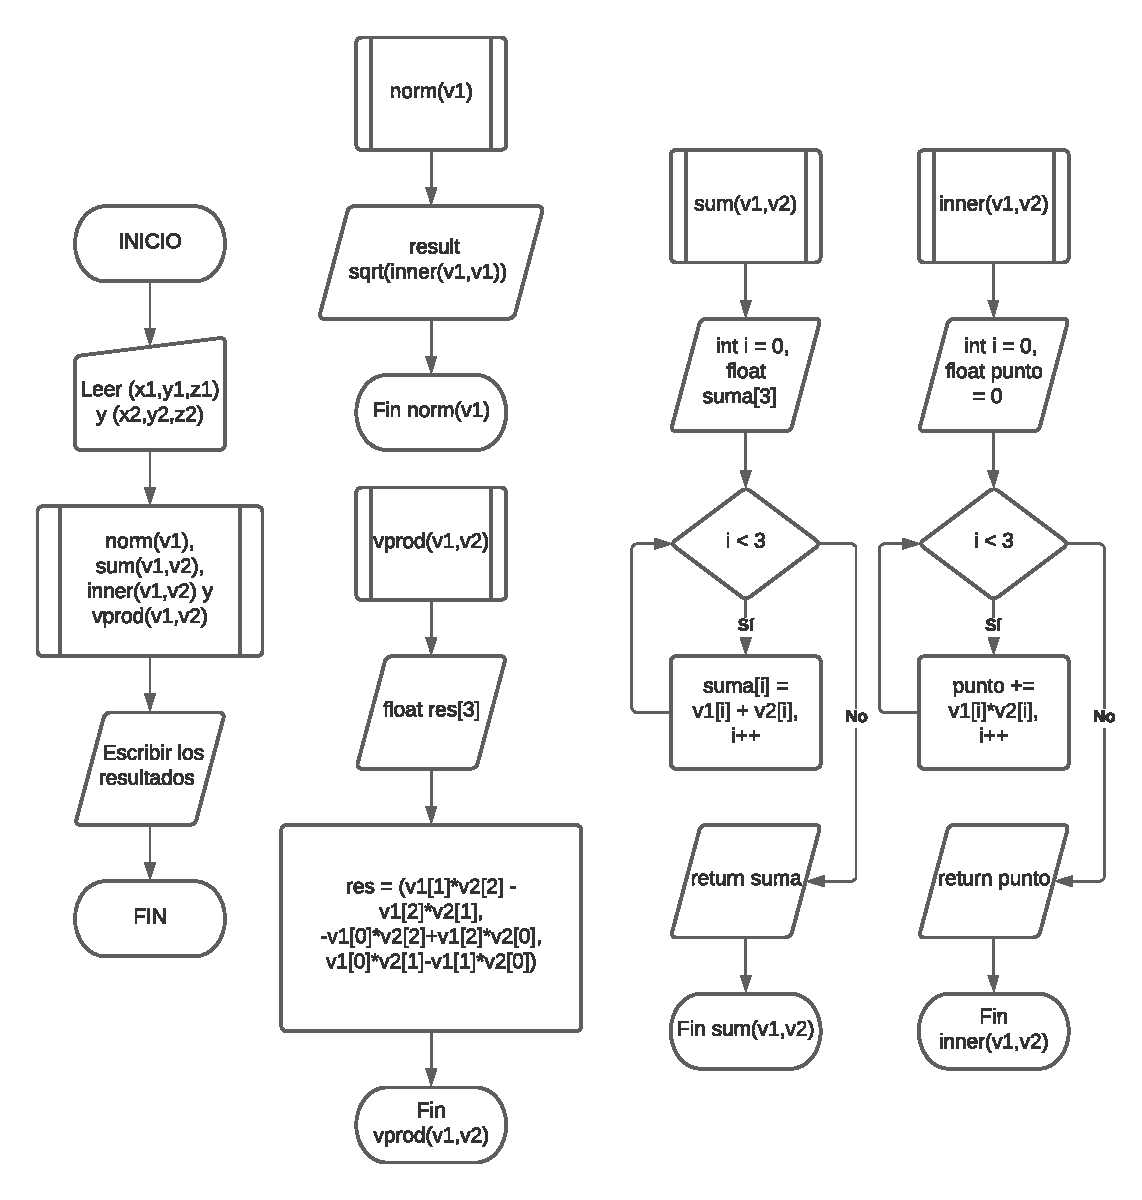
\includegraphics[scale=0.6]{img/problema3.pdf}
	\caption{Diagrama de flujo de las diferentes operaciones con vectores.}
	\label{DFp5}
\end{figure}


\subsection{Código}


\section{Problema 4}
\subsection{Enunciado}
Crear un programa que solicite al usuario dos matrices de 3X3 almacenarlas como (matA, matB) y
una constante, el programa automáticamente debe de mostrar las los siguientes resultados:
\begin{multicols}{2}
	\begin{enumerate}[a)]
		\item Matriz A por constante
		\item Suma de las matrices
		\item Resta de las matrices
		\item Multiplicación de las matrices
		\item Determinante de la matriz A
		\item Transpuesta de la matriz B
		\item Inversa de la matriz A
		\item Reducción de Gauss de la matriz A
		\item Reducción de Gauss Jordan de la matriz B
	\end{enumerate}
\end{multicols}

\subsection{Metodología}
Sean $A = (a_{ij})$ y $B = (b_{ij})$, con ambas matrices $3\times 3$ y $c\in \R$.
\begin{multicols}{2}
	\begin{enumerate}[a)]
		\item Matriz A por constante. Cada elemento de la matriz multiplicado por la constante $c$.
			$$cA = (ca_{ij}).$$
		\item Suma de las matrices. Suma elemento a elemento, es decir
			$$A + B = (a_{ij} + b_{ij}).$$
		\item Resta de las matrices. Resta elemento a elemento, i.e.
			$$A - B = (a_{ij} - b_{ij}).$$
		\item Multiplicación de las matrices. Cada elemento de la matriz resultante $\Gamma = (\gamma _ {ij})$ es de la forma
			$$\gamma _{ij} = \sum _{k = 1} ^{n = 3} a_{ik} b_{kj}.$$
		\item Determinante de la matriz A. Tomando el método de cofactores, se define el menor como el determinante de una matriz $M_{ij}$ que resulta de quitar la $i-$ésima fila y la $j-$ésima columna de la matriz original. Dado esto, se define el cofactor asociacdo a $ij$, como $\mathcal{A}_{ij} = (-1)^{i+j} M_{ij}$. Y el determinante de la matriz se calcula multiplicando cada entrada de cualquier fila (o columna) por su respectivo cofactor, es decir (tomando la fila $1$ como ejemplo)
			$$\det{A} = \sum _{j = 1} ^3 (-1)^{1 + j} a_{1j} M_{1j}.$$
		Esta fue la implementación que se quizo hacer, dado que no se pudo por problemas en el código, se utilizó la regla de Sarrus
			$$ \det{A} = \qty(a_{11}a_{22}a_{33} + a_{12}a_{23}a_{31} + a_{13}a_{21}a_{32}) $$
			$$ - \qty(a_{31}a_{22}a_{13} + a_{32}a_{23}a_{11} + a_{33}a_{12}a_{21}). $$
		\item Transpuesta de la matriz B. Se intercambian filas por columnas.
			$$B^t = (b_{ji}).$$
		\item Inversa de la matriz A. Para calcular la inversa se utiliza la siguiente relación
			$$A^{-1} = \frac{1}{\det{A}} \text{adj} (A).$$
		En donde la matriz $\text{adj} (A)$ es la matriz de cofactores transpuesta, en forma visual
			$$\text{adj} (A) = \text{cof} (A)^t = \mqty(\A _{11} & \A _{12} & \A _{13} \\ \A _{21} & \A _{22} & \A _{23} \\ \A _{31} & \A _{32} & \A _{33}) ^t.$$
		\item Reducción de Gauss de la matriz A. 
		\item Reducción de Gauss Jordan de la matriz B
	\end{enumerate}
\end{multicols}

\subsection{Variables de entrada y salida}
\begin{description}
	\item[$\rightarrow$: ] Matrices $3\times 3$ $A$ y $B$, y constante $c \in \R$.
	\item[$\leftarrow$: ] Arrays bidimensionales y constantes, cada una en relación a cada inciso.
\end{description}

\subsection{Pseudocógido o Diagrama de Flujo}
\begin{figure}[H]
\centering
\subfigure["Main"]{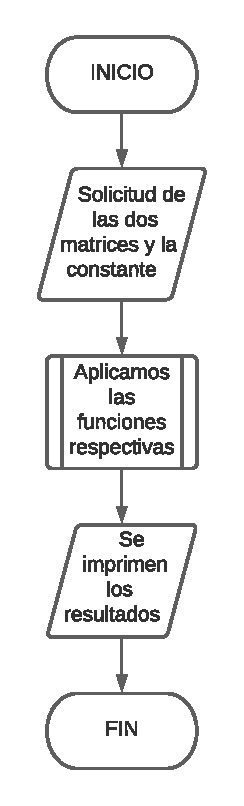
\includegraphics[scale=0.7]{img/problema4_1.pdf}}\qquad \qquad
\subfigure[Suma, resta y producto por escalar]{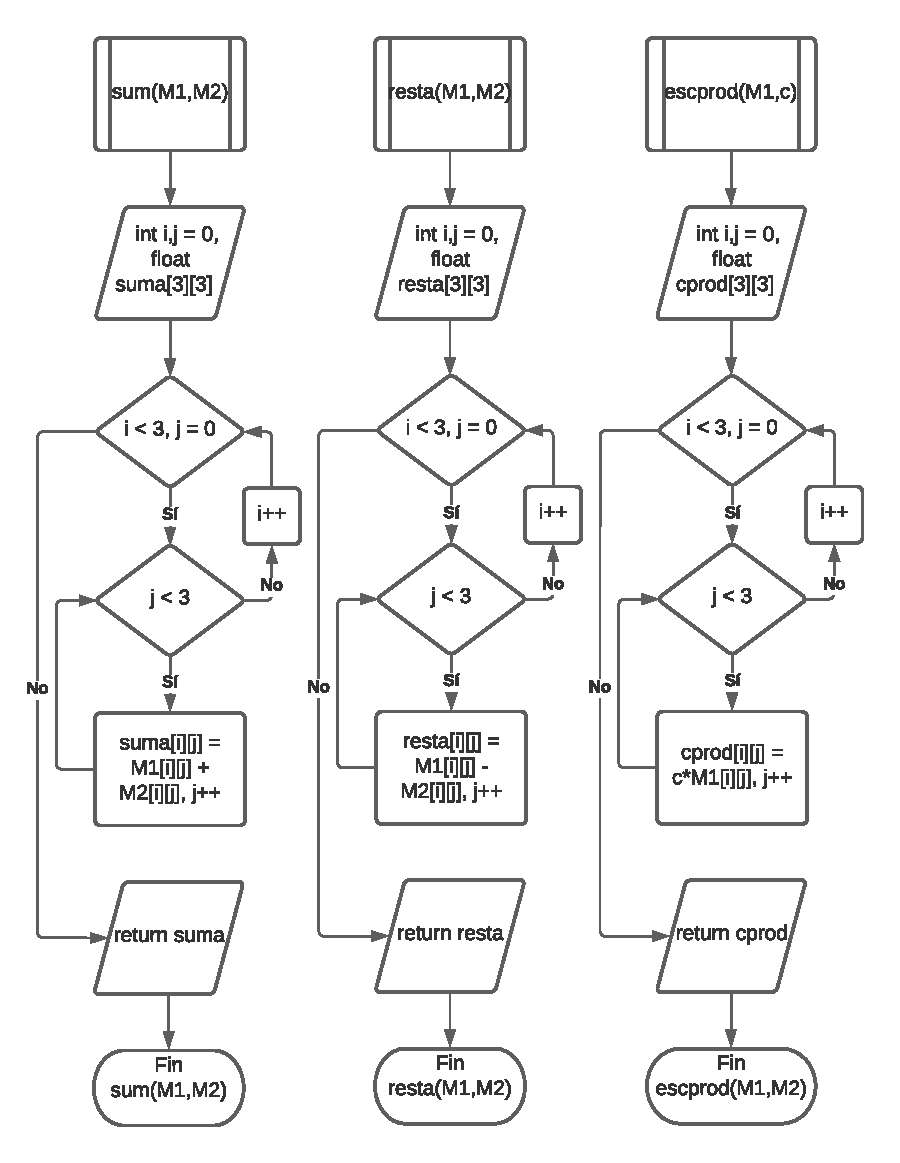
\includegraphics[scale=0.5]{img/problema4_2.pdf}}
\caption{(a) Diagrama de flujo de la función main. (b) Implementación de la suma y resta de matrices así como el producto por escalar.}
\label{FDp4}
\end{figure}

\subsection{Código}


\section{Problema 5}
\subsection{Enunciado}
Crear un programa que encuentre el factorial de un numero entero ingresado, debe de utilizar una
función recursiva.

\subsection{Metodología}
La función factorial es una función recursiva definida a tramos
	$$n! = \left\{ \mqty{n*(n-1)! & n\geq 2 \\ 1 & n = 0,1 \\ 0 & \text{en otro caso.}} \right.$$
Existen muchas otras definiciones, como la función gamma, pero para interés del problema, utilizamos la definición recursiva.

\subsection{Variables de entrada y salida}
\begin{description}
	\item[$\rightarrow$: ] Número entero $n$.
	\item[$\leftarrow$: ] Número entero. (Dado el rápido crecimiento de la función factorial, es probable que para valores, aparentemente, normales de $n$, ni siquiera los \texttt{unsigned long long int} logren poder almacenar el número.)
\end{description}

\subsection{Pseudocógido o Diagrama de Flujo}
\begin{figure}[H]
	\centering
	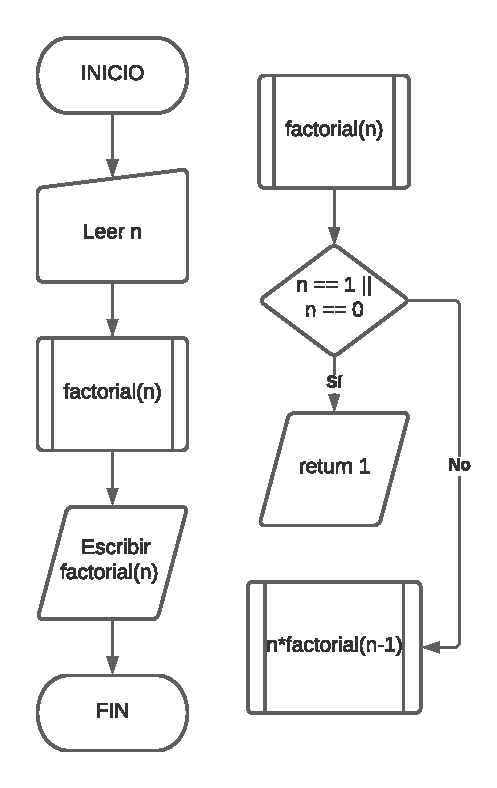
\includegraphics[scale=0.5]{img/problema5.pdf}
	\caption{Diagrama de flujo de la implementación recursiva de la función factorial.}
	\label{DFp5}
\end{figure}


\subsection{Código}


\section{Problema 6}
\subsection{Enunciado}
Crear un programa que realice la sumatoria desde 1 hasta un numero n que ingrese el usuario de las
siguientes funciones.
\begin{multicols}{2}
	\begin{enumerate}[a)]
		\item $$\sum _{k = 1} ^n k^2 (k - 3)$$
		\item $$\sum _{k = 2} ^n \frac{3}{k - 1}$$
		\item $$\sum _{k = 1} ^n \frac{1}{\sqrt{5}} \qty(\frac{1 + \sqrt{5}}{2})^k - \frac{1}{\sqrt{5}} \qty(\frac{1 - \sqrt{5}}{2})^k$$
		\item $$\sum _{k = 2} ^n 0.1(3\cdot 2^{k - 2} + 4).$$
	\end{enumerate}
\end{multicols}

\subsection{Metodología}
No hay mucho que añadir, la sumatoria es un bucle con almacenamiento en una variable que agrega el valor del paso anterior más el de la sucesión valuada en el $k$ correspondiente.

\subsection{Variables de entrada y salida}
\begin{description}
	\item[$\rightarrow$: ] Número entero $n$.
	\item[$\leftarrow$: ] Número entero o flotante, según sea el caso de la serie.
\end{description}

\subsection{Pseudocógido o Diagrama de Flujo}
\begin{description}
	\item[Paso 1: ] Prototipado de funciones para cada inciso (por simplicidad fueron nombradas con el inciso correspondiente), cuyas entradas son un número entero.
	\item[Paso 2: ] Ingreso del numero entero $n$ (limite superior de las series).
	\item[Paso 3: ] Para cada función se realizó exactamente el mismo procedimiento, solo que con diferente término de sumatoria, de modo que el ciclo for general es \\
	\texttt{Definir la suma como un float, $suma$} \\
	\texttt{Mientras un iterador sea menor igual que $n$, hacer}\\
	\texttt{suma $=$ suma $+$ $f_k$}\\
	\texttt{aumentar en $1$ el iterador}\\
	\texttt{Devolver "suma"}
	\item[Paso 4: ] Realizar esto para cada función e imprimir los respectivos resultados.
\end{description}


\subsection{Código}













%%%%%%%%%%%%5